\documentclass{article}

% if you need to pass options to natbib, use, e.g.:
%     \PassOptionsToPackage{numbers, compress}{natbib}
% before loading neurips_2024


% ready for submission
\usepackage{MPL}
\usepackage{graphicx}

% to compile a preprint version, e.g., for submission to arXiv, add add the
% [preprint] option:
%     \usepackage[preprint]{neurips_2024}


% to compile a camera-ready version, add the [final] option, e.g.:
%     \usepackage[final]{neurips_2024}


% to avoid loading the natbib package, add option nonatbib:
%    \usepackage[nonatbib]{neurips_2024}


\usepackage[utf8]{inputenc} % allow utf-8 input
\usepackage[T1]{fontenc}    % use 8-bit T1 fonts
\usepackage{hyperref}       % hyperlinks
\usepackage{url}            % simple URL typesetting
\usepackage{booktabs}       % professional-quality tables
\usepackage{amsfonts}       % blackboard math symbols
\usepackage{nicefrac}       % compact symbols for 1/2, etc.
\usepackage{microtype}      % microtypography
\usepackage{xcolor}         % colors
\usepackage{graphicx}
\usepackage{subcaption}
\usepackage{amsmath}


\title{Driver Activity Detection}

% The \author macro works with any number of authors. There are two commands
% used to separate the names and addresses of multiple authors: \And and \AND.
%
% Using \And between authors leaves it to LaTeX to determine where to break the
% lines. Using \AND forces a line break at that point. So, if LaTeX puts 3 of 4
% authors names on the first line, and the last on the second line, try using
% \AND instead of \And before the third author name.


\author{%
  Shuvam Aich \\
  Department of Computer Science\\
  University of Stuttgart\\
  Stuttgart, Germany \\
  \texttt{st187673@stud.uni-stuttgart.de} \\
  \And
  Mugdha Asgekar \\
  Department of Computer Science\\
  University of Stuttgart\\
  Stuttgart, Germany \\
  \texttt{---@stud.uni-stuttgart.de} \\
  \AND
  Prateek Chaturvedi \\
  Department of Computer Science\\
  University of Stuttgart\\
  Stuttgart, Germany \\
  \texttt{---@stud.uni-stuttgart.de} \\
  \And
  Mahdi Jafarkhani \\
  Department of Computer Science\\
  University of Stuttgart\\
  Stuttgart, Germany \\
  \texttt{st186851@stud.uni-stuttgart.de} \\
}

\begin{document}

\maketitle


\begin{abstract}
  The abstract paragraph should be indented \nicefrac{1}{2}~inch (3~picas) on
  both the left- and right-hand margins. Use 10~point type, with a vertical
  spacing (leading) of 11~points.  The word \textbf{Abstract} must be centered,
  bold, and in point size 12. Two line spaces precede the abstract. The abstract
  must be limited to one paragraph.
\end{abstract}


\section{Introduction}

\section{Project Workflow}

\section{Dataset Overview}

\section{Sliding Window}
Activity detection in videos is a challenging problem due to the continuous and dynamic nature of video data. Unlike static images, where an object classification model can predict a single label per frame, videos contain temporal dependencies where activities evolve over time.

A direct classification approach—where each frame is independently classified—often fails to capture contextual information and temporal dependencies, leading to inaccurate predictions. To address this, we employ a sliding window approach, which allows us to analyze a sequence of frames together rather than in isolation.

The key idea behind this approach is that instead of treating the entire video as a single entity or classifying individual frames separately, we use a fixed-size window that moves over the video, capturing a localized segment at each step. This enables better context preservation and helps improve detection performance.

\subsection{Motivation for Using Sliding Window}
A video typically consists of thousands of frames, and activities often span across multiple consecutive frames rather than occurring in a single instance. The sliding window approach is designed to address the following challenges:
\begin{itemize}
    \item \textbf{Temporal Overlap in Activities}: Many activities start and end gradually rather than having sharp boundaries. Using a window of frames allows the model to capture transitions effectively.
    \item \textbf{Context Awareness}: Classifying each frame in isolation lacks temporal context. The sliding window approach retains context from nearby frames, helping the model understand activity progression.
    \item \textbf{Efficiency and Performance Trade-off}: Instead of analyzing every individual frame separately (which would be computationally expensive), grouping frames into a window allows the model to process fewer but more meaningful segments.
\end{itemize}
\subsection{Implementation}
\subsubsection{Window Size and Stride}
\begin{itemize}
    \item A \textbf{fixed-size window} (e.g. 8, 16, or 32 frames) is defined, which slides across the video.
    \item The \textbf{stride} determines how much the window moves forward after each step.
    \item If the stride is \textbf{small} (e.g., 1 frame), the overlap between windows increases, leading to \textbf{better temporal coverage but higher computational cost}.
    \item If the stride is \textbf{large} (e.g., 8 frames), fewer windows are processed, reducing computation but potentially \textbf{missing fine-grained transitions}.
\end{itemize}

\subsubsection{Processing Each Window}
\begin{itemize}
    \item Each window of frames is sent as input to a pre-trained I3D model.
    \item The model infers on the window and predicts the most likely activity to occur in that segment.
    \item The predicted label is assigned to each frame of the window, along with the confidence scores (Figure \ref{fig:sliding-window-predictions}).
    \item The activity with the highest confidence score is selected for each frame.
    \item As the window progresses, new predictions are generated, leading to a continuous activity timeline.
\end{itemize}

\begin{figure}[h]
    \centering
    \begin{subfigure}{0.45\textwidth}
        \centering
        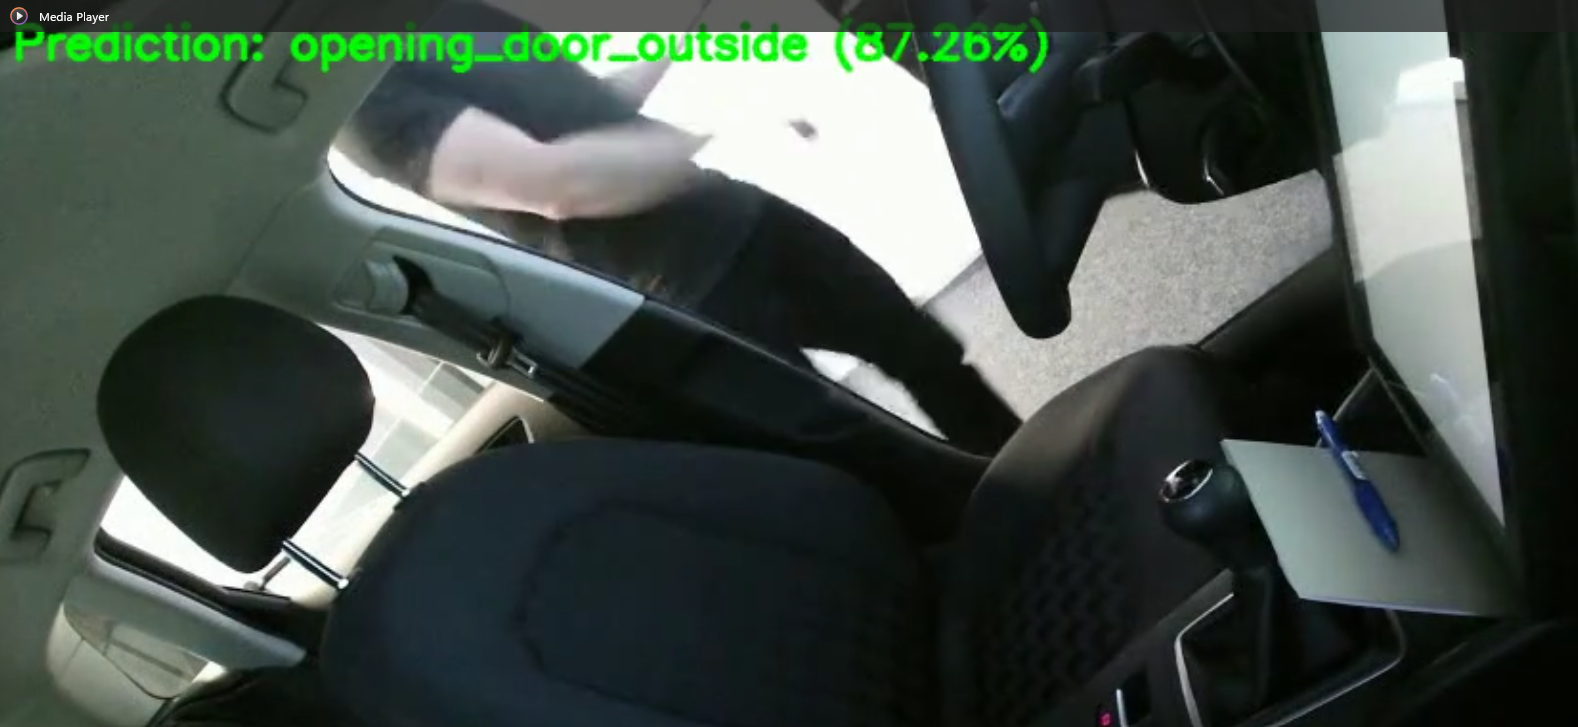
\includegraphics[width=\textwidth]{figs/DAR1.png}
        \caption{Opening door outside}
    \end{subfigure}
    \hspace{0.5cm}
    \begin{subfigure}{0.45\textwidth}
        \centering
        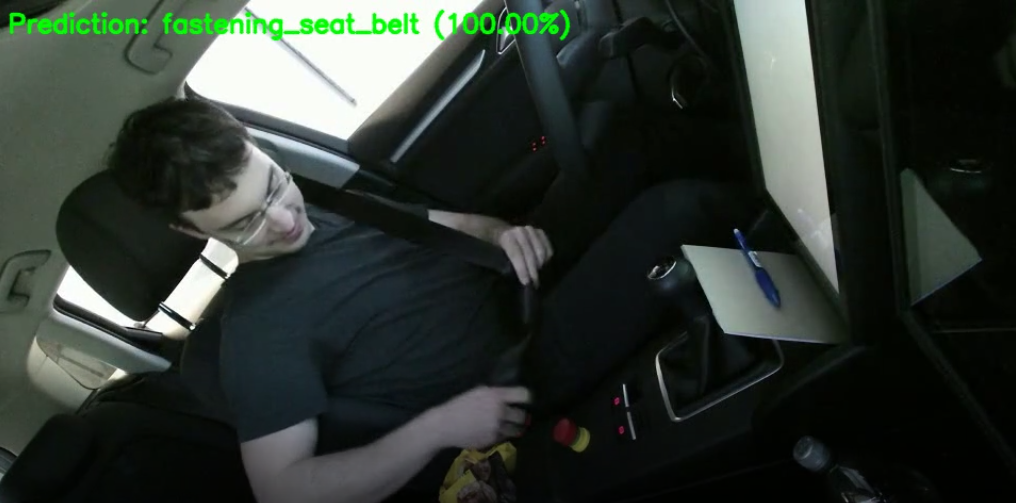
\includegraphics[width=\textwidth]{figs/DAR2.png}
        \caption{Fastening Seat Belt}
    \end{subfigure}

    \vspace{0.5cm}

    \begin{subfigure}{0.45\textwidth}
        \centering
        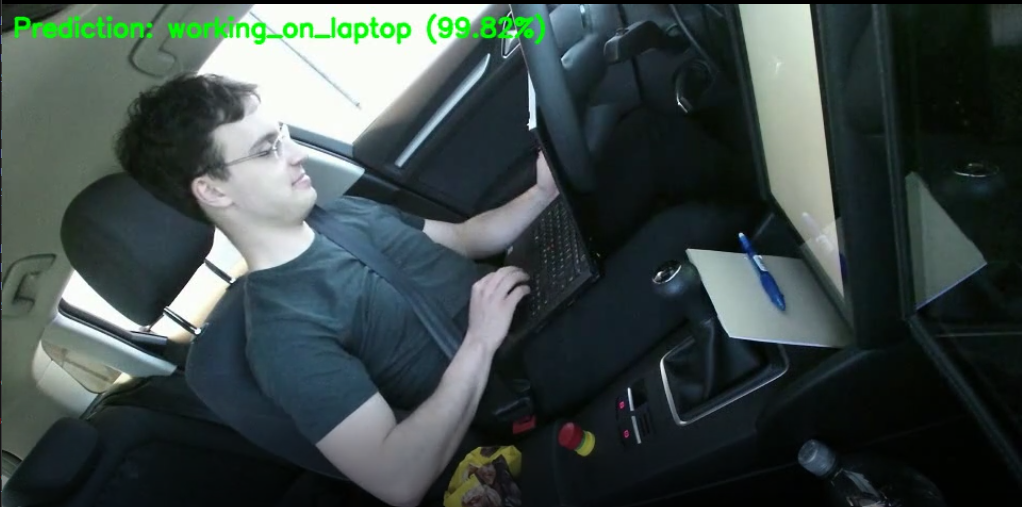
\includegraphics[width=\textwidth]{figs/DAR3.png}
        \caption{Working on Laptop}
    \end{subfigure}
    \hspace{0.5cm}
    \begin{subfigure}{0.45\textwidth}
        \centering
        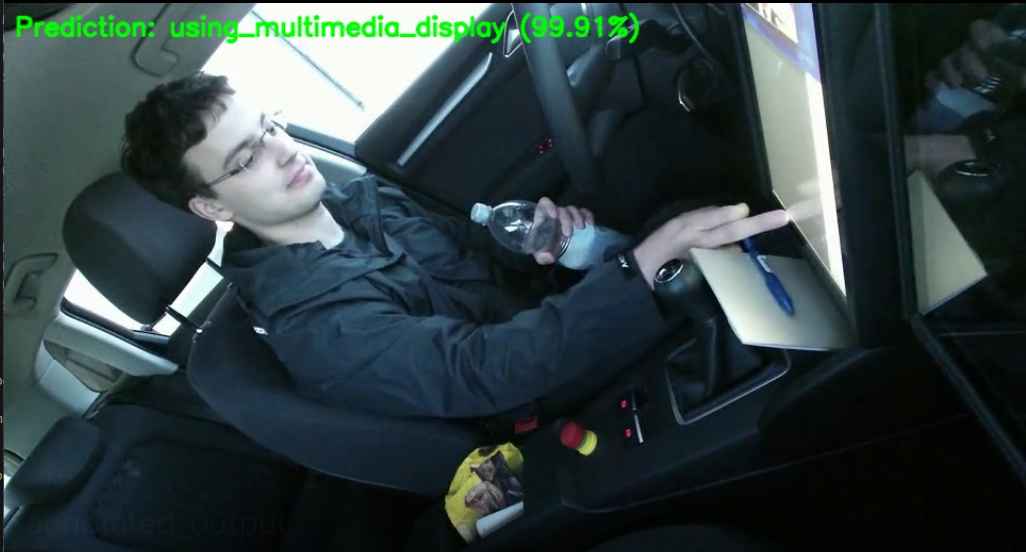
\includegraphics[width=\textwidth]{figs/DAR4.png}
        \caption{Using Multimedia Display}
    \end{subfigure}

    \caption{Grid for multiple predictions using Sliding Window.}
    \label{fig:sliding-window-predictions}
\end{figure}

\section{Metrics}
Evaluating activity detection models requires quantitative metrics that measure how well predictions align with ground truth activities. One of the objectives involved was to develop metrics for the sliding window approach to understand how accurate are the predictions. We employ two key metrics as mentioned in the next sections.

\subsection{Midpoint Hit Criteria}

To determine whether a prediction is correct, we used the \textbf{midpoint hit criteria}. For each ground truth activity segment, we computed its midpoint and checked if a predicted segment of the same activity class covered this midpoint. The evaluation steps are as follows:

\begin{itemize}
    \item Compute the \textbf{midpoint} of each ground truth segment as:
    \begin{equation}
        \text{midpoint} = \frac{\text{frame\_start} + \text{frame\_end}}{2}
    \end{equation}
    \item A prediction is counted as a \textbf{true positive (TP)} if it covers the midpoint and belongs to the correct activity class.
    \item If no prediction matches the midpoint, it is considered a \textbf{false negative (FN)}.
    \item Any extra predicted segments that do not match a ground truth midpoint count as \textbf{false positives (FP)}.
    \item Precision and recall for each activity class are calculated as:
    \begin{equation}
        \text{Precision} = \frac{TP}{TP + FP} \times 100
    \end{equation}
    \begin{equation}
        \text{Recall} = \frac{TP}{TP + FN} \times 100
    \end{equation}
    \item Overall precision and recall are computed by aggregating across all activity classes.
\end{itemize}

\subsection{Intersection over Union (IoU)}

To measure how well the predicted activity windows overlap with the ground truth, we used \textbf{IoU}:

\begin{itemize}
    \item \textbf{Intersection}: The overlapping frames between the ground truth and predicted segment.
    \item \textbf{Union}: The total number of frames covered by both segments.
    \item The IoU score for each ground truth segment is calculated as:
    \begin{equation}
        \text{IoU} = \frac{\text{Intersection}}{\text{Union}}
    \end{equation}
    \item The \textbf{mean IoU} is obtained by averaging the IoU scores across all ground truth segments.
\end{itemize}

\subsection{Final Evaluation Results}

The model outputs the following results:

\begin{itemize}
    \item \textbf{Precision per class (\%)}: Precision values for each activity class.
    \item \textbf{Recall per class (\%)}: Recall values for each activity class.
    \item \textbf{Overall Precision}: Aggregated precision across all activities.
    \item \textbf{Overall Recall}: Aggregated recall across all activities.
    \item \textbf{Mean IoU}: The average IoU score across all activity segments.
\end{itemize}

These metrics provide a comprehensive evaluation of the accuracy and localization performance of the model.

\section{Neural Detection Model}
Manuel and Roitberg \cite{drive_and_act_2019_iccv} evaluated various models for fine-grained driver activity recognition using the DriveAndAct dataset. They tested different approaches, including CNN-based methods (like C3D, P3D ResNet, and I3D) and body pose-based methods. They found out that the Inflated 3D ConvNet (I3D), an extension of the Inception-v1 network with 3D convolutions, achieved the highest accuracy (69.57\% on Validation, and 63.64\% on test) among all tested models for recognizing fine-grained driver activities.
I3D also outperformed body pose-based methods, which were less effective in classifying actions despite incorporating spatial and temporal streams.
In atomic action unit classification, I3D performed best in recognizing actions (56.07\%) and objects (56.15\%), though body pose-based approaches were better at identifying locations (56.5\%).Although for cross-view action recognition, I3D models struggled with domain shifts, performing significantly worse when tested on unseen views.
\subsection{I3D Model}
The Two-Stream Inflated 3D ConvNet (I3D) \cite{carreira2018quovadisactionrecognition} is a deep learning model designed for video action recognition. It extends 2D convolutional neural networks (CNNs) into 3D by "inflating" their filters and pooling kernels to operate in both spatial and temporal dimensions. This allows the model to effectively capture motion patterns in videos (Figure \ref{fig:i3d}).
\subsubsection{Key Features of I3D}
\begin{itemize}
    \item \textbf{3D Convolutions}: Unlike traditional 2D CNNs that process images independently, I3D uses 3D convolutional layers to extract spatiotemporal features from videos.
    \item \textbf{Inflation from 2D Networks}: The model is based on the Inception-v1 architecture, with its 2D filters expanded into 3D. This allows it to reuse ImageNet pre-trained weights, improving efficiency and performance.
    \item \textbf{Two-Stream Configuration}: I3D processes both RGB frames (spatial information) and Optical flow (motion information). These two streams are trained separately and their outputs are fused at the end.
\end{itemize}

\begin{figure}[h]
    \centering
    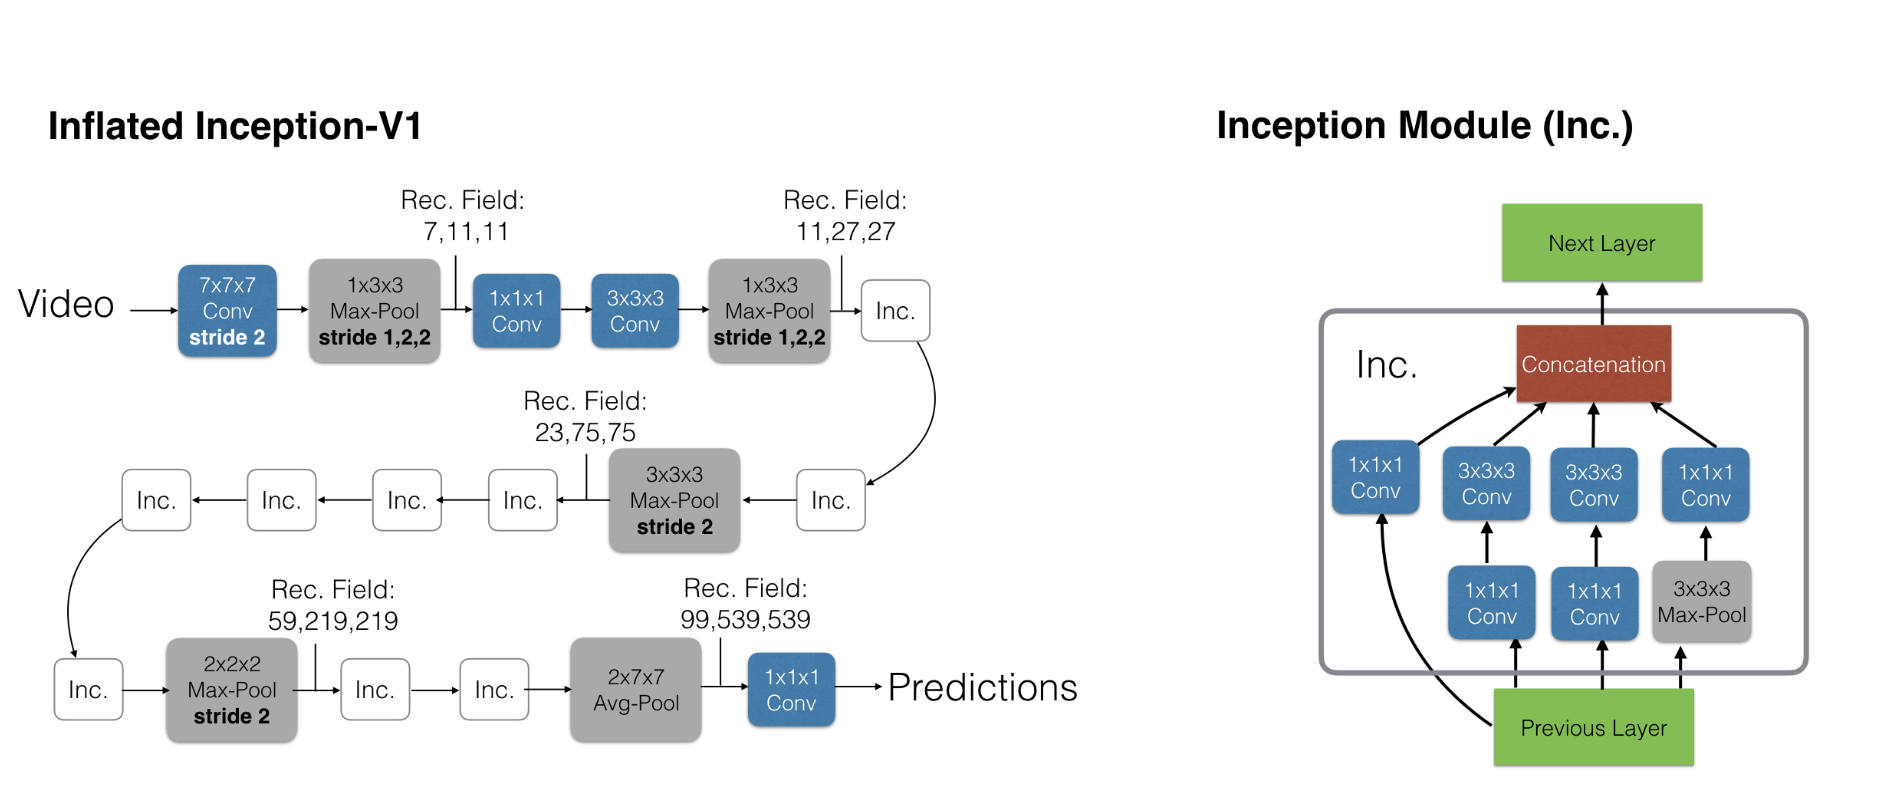
\includegraphics[width=0.8\linewidth]{figs/i3d.png}
    \caption{The Inflated Inception-V1 architecture (left) and its detailed inception submodule (right). The strides of convolution and pooling
operators are 1 where not specified, and batch normalization layers, ReLu’s and the softmax at the end are not shown. The theoretical
sizes of receptive field sizes for a few layers in the network are provided in the format “time,x,y” – the units are frames and pixels. The
predictions are obtained convolutionally in time and averaged.\cite{carreira2018quovadisactionrecognition}}
    \label{fig:i3d}
\end{figure}

\subsection{I3D Model as baseline model}
We utilized the I3D model for recognition in our project. We evaluated a pre-trained I3D model and performed inference on all videos in the Kinetic Color category. Figure \ref{fig:i3d-acc} illustrates the model's accuracy on the DriveAndAct dataset. The dataset includes 15 viewpoints, each comprising two runs, except for viewpoint 9, which lacked annotation for the second run. The average accuracy is 82.26\% for our baseline model.
We noticed the main reason for misclassfying each frame to its action is either by:
\begin{itemize}
    \item \textbf{Latency in Annotation}: Since human-labeled annotations (ground truths) lack a strict consensus on the exact start time of an action, some degree of misclassification is inevitable. In this context, misclassifying an action by at most 10 frames is considered acceptable or, in other words, irreducible.
    \item \textbf{Fast Switching Actions}: The model exhibited rapid transitions between actions, sometimes within less than 3 frames. This behavior was of particular interest to us, and we hypothesized that applying a neural network or transformer architecture on top of the I3D model could help reduce this misclassification.
\end{itemize}
\begin{figure}[h]
    \centering
    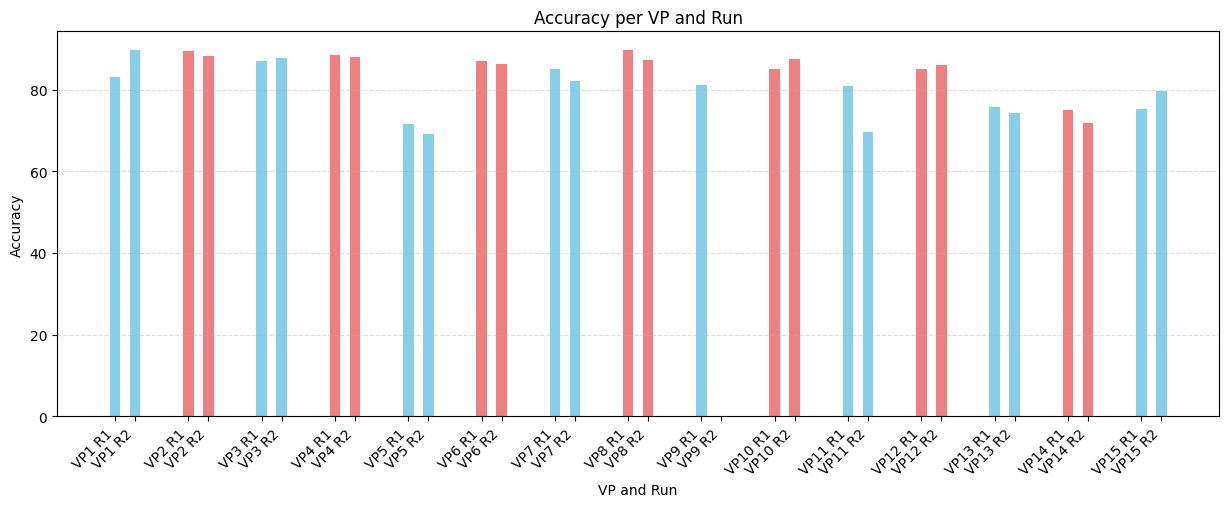
\includegraphics[width=0.8\linewidth]{i3d-acc.png}
    \caption{Accuracy for recognition task with I3D model on all viewpoints and runs on Kinetic Color category, DriveAndAct dataset}
    \label{fig:i3d-acc}
\end{figure}
\subsection{Extending I3D Model}
\subsubsection{Preprocessing}
The input data utilized in this study was originally trained using the I3D model, which generated class probabilities as output. These probabilities were stored in .pt files for subsequent processing. To prepare the data for our detection model, we computed the argmax of the arrays containing the class probabilities, thereby converting them into discrete class labels. These labels were then used as input for training the detection model.

Due to computational constraints, we processed each video in the dataset individually. The training dataset consisted of 19,071 frames, with each frame represented by an array of 34 class probabilities. Frame-wise annotations were stored in corresponding CSV files, where missing annotations were denoted by a placeholder value of 40.

The preprocessing phase involved converting the class probabilities into discrete labels using the numpy argmax function. Additionally, batch processing techniques were employed to optimize memory usage, ensuring efficient handling of large datasets during training and inference. This approach facilitated the effective training of the detection model while mitigating computational limitations.
\subsubsection{Model Enhancements and Challenges}
To enhance accuracy, several advanced model architectures were explored, including transformers, temporal convolutional neural networks (CNNs), and recurrent neural networks (RNNs). A major challenge encountered was aligning the input and target dimensions for loss computation. Additionally, batch size mismatches and tensor shape inconsistencies required careful debugging and adjustments to the data pipeline. Some approaches achieved high training accuracies; however, test accuracy remained significantly lower.

To stabilize training and mitigate overfitting, techniques such as early stopping and batch normalization were implemented. Early stopping prevented unnecessary overtraining by halting training once validation performance plateaued; however, accuracy did not improve. Increasing the training data and performing hyperparameter tuning also had minimal impact. In some cases, modifications to the model architecture even reduced the accuracy of the training.

The transformer-based architecture uses an embedding layer, positional encoding, a stack of Transformer encoder layers, and a final linear layer for classification. If the model needs to consider the entire sequence (e.g., correlations across distant frames), the transformer should excel hence this approach. Training was faster because the sequence is processed as a whole rather than step by step and the self-attention mechanism captured long-range relationships more effectively. However, our training accuracy was very low indicating that our model was not able to learn the features properly.

The Long Short-Term Memory (LSTM) model was configured with one layer. This vanilla LSTM does not include attention mechanisms, which allow the model to selectively focus on specific time steps rather than relying only on the last hidden state. Stacked LSTMs, which use multiple layers, can model more complex temporal hierarchies but come at a higher computational cost. This vanilla LSTM does not include attention mechanisms, which allow the model to selectively focus on specific time steps rather than relying only on the last hidden state. While the LSTM demonstrated promise in capturing temporal relationships within the data, tuning its hyperparameters (e.g., number of layers, hidden units, and learning rate) was critical for optimization. Despite these efforts, overfitting remained a challenge, particularly on smaller subsets of data, necessitating further exploration of regularization techniques. One model configuration achieved a high training accuracy but a very low test accuracy. The best-performing approach, with additional data manipulations, showed negligible improvement. This study does not claim the approach to be entirely correct, as it involved experimental exploration of both the data, the inputs and the models.
\section{Conclusion}

\bibliographystyle{alpha}
\bibliography{MPL}

\end{document}